\chapter{System configuration and assessment} \label{chap:results}

With the complete system running, it is now possible to discuss the results of the proposed system. In this chapter, we will discuss not only the results obtained, but also the preprocessing steps that were taken in order to obtain them, and the testing methodology that was used in order to conduct the perceptual tests. The results will be discussed in the context of the proposed system architecture, and the whisper activity detection and speech segmentation algorithms that were used in the proposed system for silence detection and Voiced/Unvoiced decisions.

\section{Dataset and Preprocessing}

For the data, the original DyNaVoiceR dataset \cite{JESUS2023101223} was utilized, which is a matched dataset of both voiced and whispered speech utterances that were recorded within a controlled environment in a soundproof room and high quality recording equipment \cite{castilho2019fct}. The database consisted of 13 sustained sounds, i.e. vowels and sibilants from european portuguese, 28 words, 6 short phrases and a small text. These were uttered by 30 speakers, with an equal representation of male and female genders. From this, a smaller subset of just 4 samples of two phrases from different speakers was done, in order to test the proposed system.

\begin{table}[H]
    \centering
    \begin{tabular}{cc}
        \hline
        Test Phrase & Speaker \\
        \hline \hline
        \multirow{2}*{\textit{A asa do avião andava avariada}} & SPF05 \\
        & SPM18 \\
        \hline
        \multirow{2}*{\textit{O tiago comeu quatro pêras}} & SPF12 \\
        & SPM14 \\
        \hline
    \end{tabular}
    \caption{Samples user for testing}
    \label{tab:dataset}
\end{table}

\subsection{Fundamental Frequency Analysis}

In order to maximize the quality of the comparisons between converted whispered speech and the reference samples, the fundamental frequency of the reference samples was analyzed in order to obtain the average fundamental frequency of each sample. This was achieved by means of the probabilist Yin algorithm \cite{mauchPYINFundamentalFrequency2014}, which is a robust and efficient algorithm for monophonic fundamental frequency estimation. Librosa provides this algorithm as a function \texttt{pyin()} \cite{mcfee_2024_11192913}, which was used to analyze the fundamental frequency of the reference samples, the results of which are shown in Figure \ref{fig:f0analysis}.

\begin{figure}[H]
    \centering
    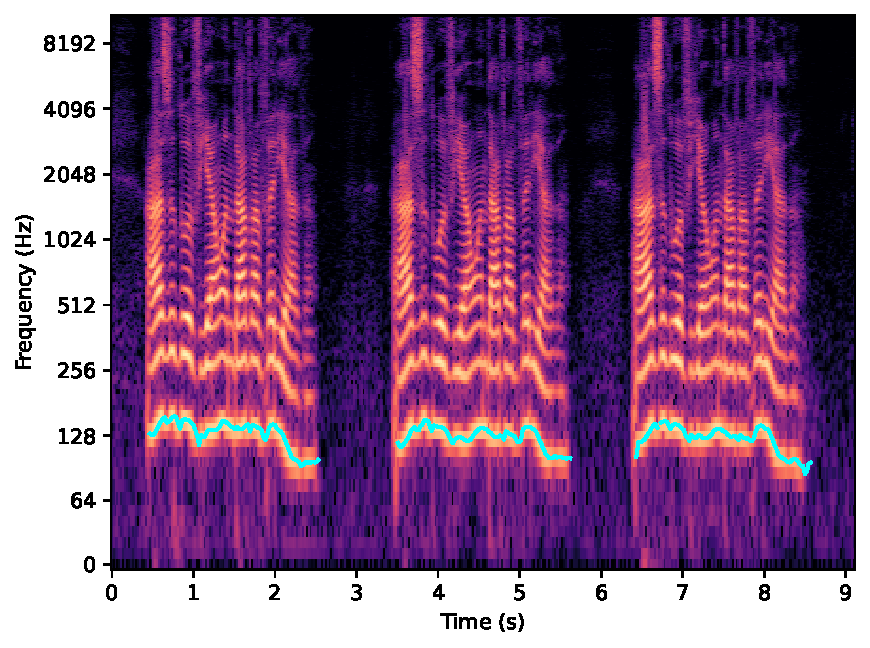
\includegraphics[width=0.75\textwidth]{chapter7/f0analysis.pdf}
    \caption{Fundamental frequency analysis of a voiced reference sample - Subject SPM18}
    \label{fig:f0analysis}
\end{figure}

\subsection{Noise Removal and Audio Restoration}

Due to the nature of the dataset and the recording methodology chosen, the whispered speech was recorded with a much higher gain than the voiced speech, which made it necessary to preprocess all whispered samples in order to remove background noise. Also, due to the higher gain, the whispered samples had much more clicking and slight popping sounds, due to lips and tongue smacking, which also had to be removed. For this, Adobe Audition 2024 was used to attenuate both of these.

First the noise was removed using the noise reduction effect, by first selecting a portion of the audio that was just noise (i.e. no whispered speech nor breathing) and then applying the noise reduction effect with the automatic settings. These proved to be quite effective at removing most of the noise that interfered with the whispered speech detection and segmentation algorithms. After this, the clicking sounds were removed with the Click/Pop Eliminator process \cite{adobe_audition_noise_reduction}, with the settings set empirically on a sample-by-sample basis, in order to remove the clicking sounds without affecting the whispered speech.

Besides this, the audio was normalized to not exceed -12dB, in order to avoid clipping and to ensure that the converted audio samples would remain in the same loudness range in relation to the reference and each other. For this, Ableton Live 11 was used, with a limiter applied to all audio samples with a gain of +6dB and a ceiling of -12dB, using automatic lookahead and release settings. 

\section{Testing Environment}

In order to gather the perceptual data for the proposed system, a MUSHRA listening test was conducted with responses from 17 volunteers, with ages ranging from 22 to 61. Multiple Stimuli with Hidden Reference and Anchor (MUSHRA) \cite{internationaltelecommunicationunionBS15343Method2015} is a testing methodology that is widely used in audio and speech quality assessment, where listeners are asked to rate and compare the quality of different audio samples. It works by presenting the listener with a set of audio samples, where one of them is a reference sample, and the listener is asked to rate the quality of other samples in relation to the reference.

Considering this, a testing environment was deployed using the open source platform webMUSHRA platform \cite{schoefflerWebMUSHRAComprehensiveFramework2018}. This was in turn deployed using PyMushra which is yet another open-source project that is meant to simplify the deployment of the webMUSHRA framework, by providing a simple Flask web server and a tinydb database for the storage of the results. This last python package also supports exporting the data results directly to a python environment as a Pandas dataframe, allowing for quick statistical analysis using SciPy and visualization using Seaborn.


\subsection{Whispered-to-Speech Conversion}

As mentioned in the previous chapter, the tests that are conducted in terms of whispered to speech conversion are first implemented using individual pulse filtering as per the scheme in Figure \ref{fig:pulseMap} and another one by computing one filter per frame, so as to obtain an idea of the improvement that the filter interpolation mechanism brings to the system. In comparison, we will have the complete system using the activity detection, speech segmentation and $F_0$ contour, in order to evaluate the improvement in prosody and overall quality that these mechanisms contribute in terms of conversion. The parameters that were used for the whispered-to-speech conversion are shown in table \ref{tab:w2cSettings}.


\begin{table}[H]
    \centering
    \begin{tabular}{cccc}
        \hline
        Speaker & $F_{vuv}$ (Hz) & $F_{uv}$ (Hz) & Avg. $F_0$ (Hz)\\
        \hline \hline
        SPF05 & 2400 & 3400 & 191.65 \\ \hline 
        SPF12 & 2400 & 3400 & 165.33 \\ \hline
        SPM14 & 1800 & 2400 & 111.30 \\ \hline
        SPM18 & 1800 & 2400 & 127.60 \\ \hline
    \end{tabular}
    \caption{\centering Centre of gravity thresholds and average fundamental frequency \\ for each of the converted samples}
    \label{tab:w2cSettings}
\end{table}

The testing page is shown in Figure \ref{fig:mushraW2C}, where the user is presented with the reference sample, the converted sample and a feedback form. Here, the test subject is presented with the reference voiced audio and 5 randomized stimuli samples. These are: the hidden reference, the original whispered audio, the full system conversion and the two intermediary steps of individual pulse filtering and frame-by-frame filtering. The latter is presented as representation of the EL, which is compared with the individual pulse filtering and the segmented conversion. Table \ref{tab:w2cConditions} provides a brief description of the test conditions that were used for the whispered-to-speech conversion tests.

\begin{table}[H]
    \centering
    \begin{tabular}{p{0.2\textwidth}p{0.6\textwidth}}
        \hline 
        Test Condition & Description \\
        \hline \hline
        Reference & Voiced reference sample \\
        Whispered & Original whispered sample \\
        Frame Filtering & WSC using a single filter for each audio segment \\
        Pulse Filtering & WSC using filtering for each individual glottal pulse\\
        Complete System & WSC using pulse filtering, along with the $F_0$ contour, silence detection using WAD and segmentation with V/UV decisions \\
        \hline
    \end{tabular}
    \caption{Whispered-to-Speech conversion test conditions}
    \label{tab:w2cConditions}
\end{table}
    
The user is then asked to rate the samples in terms of how intelligible and natural it sounds, and how good the audio samples are in terms of overall quality. A scale is provided where the scores are labeled in the following manner: 0-20 is bad, 20-40 poor, 40-60 fair, 60-80 good and 80-100 is excellent.

\subsection{Vowel synthesis}

Another test was conducted in order to evaluate how natural the pulse generation and the filtering mechanisms presented in Chapters \ref{chap:pulseGen} and \ref{chap:filt}, respectively, are in terms of vowel synthesis. Here the reference is the original voiced vowel, and the stimuli are the completely synthesized vowels along with the reference. In the former case, two types of vowels are generated, one with a constant $F_0$ frequency and the other following the $F_0$ contour that was established in Chapter \ref{chap:pulseGen}.

All five vowels were then concatenated into a single audio file for each stimuli, and the user was asked to rate the samples in the same manner as the whispered-to-speech conversion test. The testing page is shown in Figure \ref{fig:mushraVowel}.  

\section{Results and Discussion}

The results of all tests are presented in the following subsections. For all tests, all recorded data points were used, and the results were analyzed using the mean, variance and the bilateral 95\% confidence interval. Also paired t-tests were conducted in order to determine if the differences between the results were statistically significant, with a significance level (p-value) of 0.05.

\subsection{Whispered-to-Speech Conversion}

Figures \ref{fig:w2sTiago} and \ref{fig:w2sAviao} show the results of the whispered-to-speech conversion tests for the phrases \textit{"O Tiago comeu quatro pêras"} and \textit{"A asa do avião andava avariada"}, respectively, presented in a box and whisker plot indicating the distribution of each quartile of data. All data points are also shown in the plot as the gray dots, along with white circles that indicate outliers. The other results from statistical analysis are presented in Table \ref{tab:w2s}.

\begin{figure}[H]
    \centering
    \begin{minipage}[H]{0.495\textwidth}
        \centering
        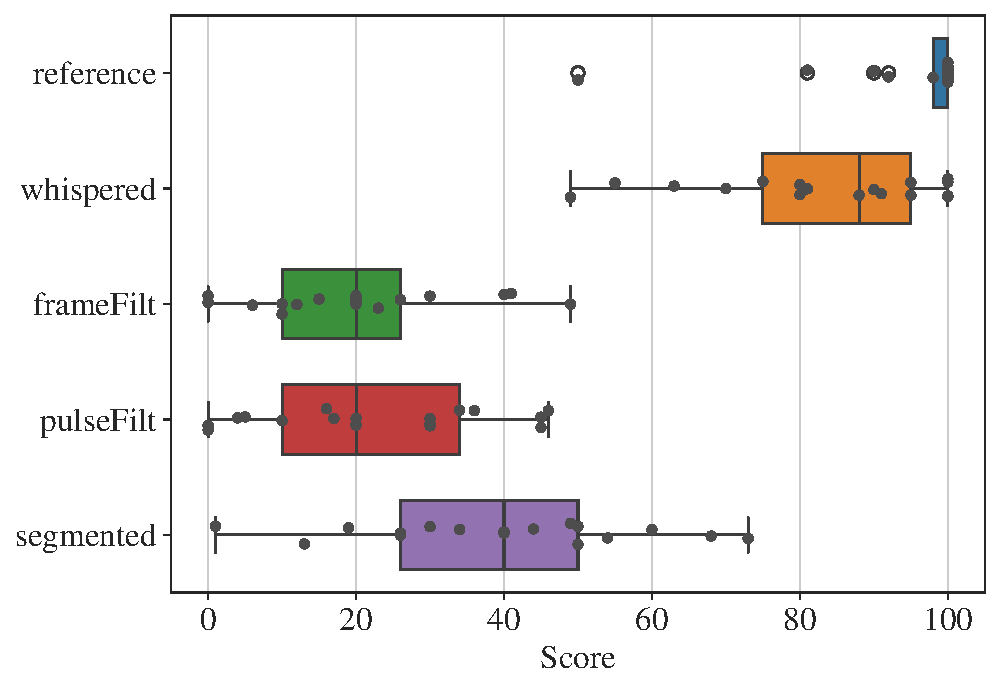
\includegraphics[width=\textwidth]{chapter7/SPF05_aviao.pdf}
        \subcaption{SPF05}
    \end{minipage}
    \begin{minipage}[H]{0.495\textwidth}
        \centering
        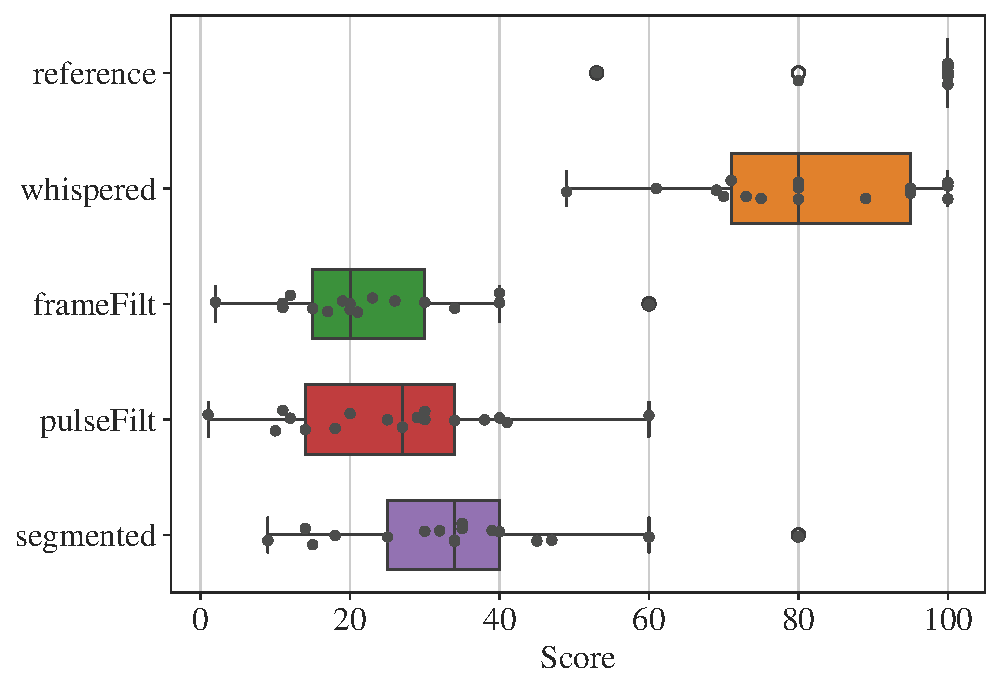
\includegraphics[width=\textwidth]{chapter7/SPM14_tiago.pdf}
        \subcaption{SPM14}
    \end{minipage}
    
    \caption{\centering Whispered-to-Speech conversion results - \\ \textit{"O Tiago comeu quatro pêras"}}
    \label{fig:w2sTiago}
\end{figure}

\begin{figure}[H]
    \centering
    \begin{minipage}[H]{0.495\textwidth}
        \centering
        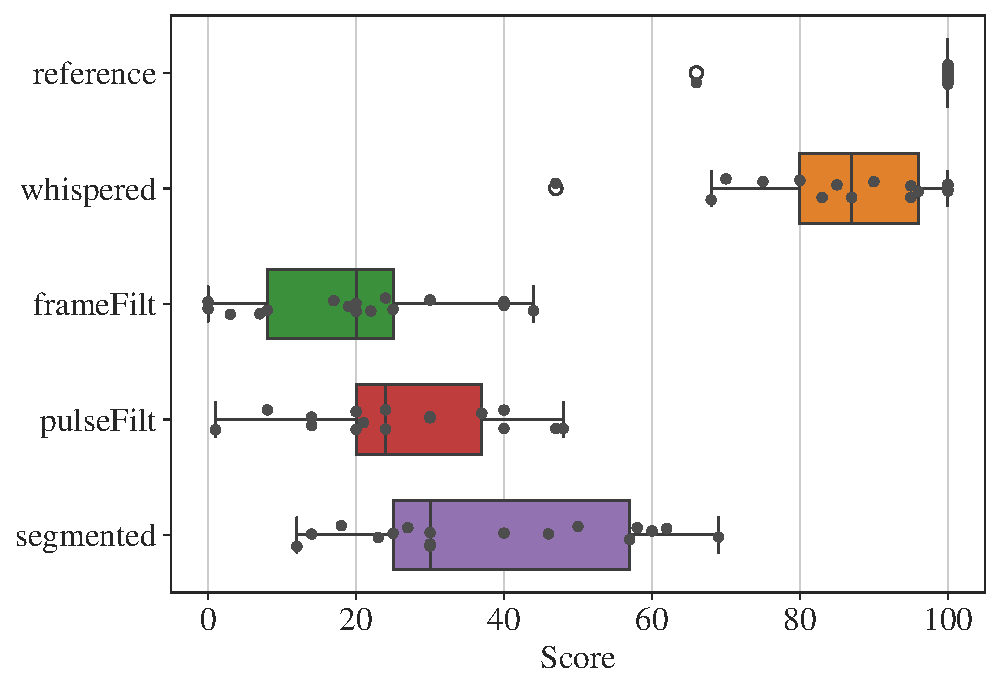
\includegraphics[width=\textwidth]{chapter7/SPF12_tiago.pdf}
        \subcaption{SPF12}
    \end{minipage}
    \begin{minipage}[H]{0.495\textwidth}
        \centering
        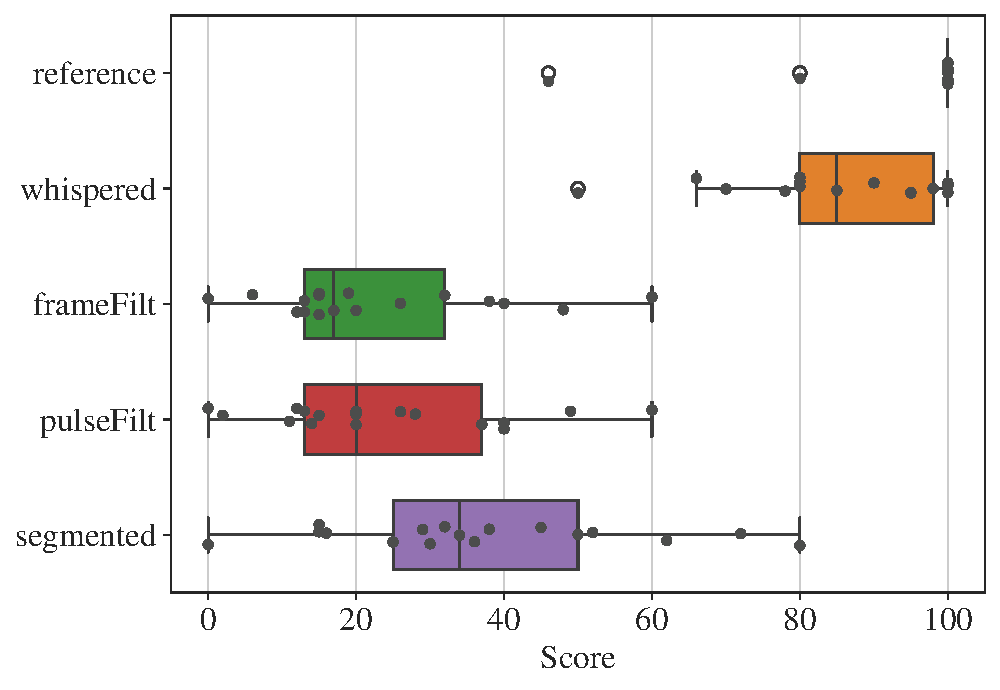
\includegraphics[width=\textwidth]{chapter7/SPM18_aviao.pdf}
        \subcaption{SPM18}
    \end{minipage}
    \caption{\centering Whispered-to-Speech conversion results - \\ \textit{"A asa do avião andava avariada"}}
    \label{fig:w2sAviao}
\end{figure}

The results show that the complete system is able to outperform the individual pulse filtering and frame filtering mechanisms, with higher mean scores than both. This does show that the proposed system is able to generate more natural sounding speech that these other two steps, which is in line with the expectations. Both the frame filtering and individual pulse filtering represent naturalness and intelligibility levels akin to that of a EL device, showing that the effect of both segmentation and $F_0$ contour has quite a significant impact in the conversion process.

By doing a paired t-test, as shown in Tables \ref{tab:pairwiseSPF05}, \ref{tab:pairwiseSPF12}, \ref{tab:pairwiseSPM14} and \ref{tab:pairwiseSPM18}, it was found that the differences were statistically significant for all samples, except for the comparison between the individual pulse filtering and the frame filtering where p > 0.05, indicating that the differences between these two are not statistically significant. Despite this, the means between these two are slightly different, with the pulse-wise filtering having a slightly higher mean than the frame-wise mechanism, which is in line with the expectations.

The main reason for this is that the hard filter changes that are done by computing a filter per frame, are not as smooth and introduce a spring reverb-like periodic artifact that is noticeable after long periods of listening. This is not present in the individual pulse filtering mechanism, which is able to generate a smoother and more natural sounding speech, as the filter is computed for each pulse and then interpolated between them.

\begin{table}[H]
    \centering
    \begin{tabular}{crcccc}
        \hline
         & & SPF05 & SPF12 & SPM14 & SPM18 \\ \hline

        \multicolumn{1}{l|}{\multirow{3}*{Reference}} & $\mu$ & 94.765 & 98.000 & 96.059 & 95.647 \\ %\cline{2-6}
        \multicolumn{1}{l|}{} & $\sigma^2$ & 12.657 & 8.246 & 12.106 & 13.679 \\ 
        \multicolumn{1}{l|}{} & $CI_{95\%}$ & $\pm$ 6.02 & $\pm$ 3.92 & $\pm$ 5.75 & $\pm$ 6.50\\ \hline

        \multicolumn{1}{l|}{\multirow{3}*{Whispered}} & $\mu$ & 83.059 & 85.353 & 81.588 & 85.118 \\ %\cline{2-6}
        \multicolumn{1}{l|}{} & $\sigma^2$ & 16.157 & 14.491 & 15.383 & 14.260 \\ 
        \multicolumn{1}{l|}{} & $CI_{95\%}$ & $\pm$ 7.68 & $\pm$ 6.89 & $\pm$ 7.31 & $\pm$ 6.78 \\ \hline

        \multicolumn{1}{l|}{\multirow{3}*{Complete System}} & $\mu$ & 39.824 & 38.294 & 34.823 & 37.118 \\ %\cline{2-6}
        \multicolumn{1}{l|}{} & $\sigma^2$ & 19.340 & 18.289 & 17.458 & 21.254 \\ 
        \multicolumn{1}{l|}{} & $CI_{95\%}$ & $\pm$ 9.19 & $\pm$ 8.69 & $\pm$ 8.30 & $\pm$ 10.10 \\ \hline

        \multicolumn{1}{l|}{\multirow{3}*{Pulse Filtering}} & $\mu$ & 22.824 & 25.765 & 25.882 & 23.941 \\ %\cline{2-6}
        \multicolumn{1}{l|}{} & $\sigma^2$ & 15.709 & 13.339 & 14.521 & 16.479 \\ 
        \multicolumn{1}{l|}{} & $CI_{95\%}$ & $\pm$ 7.45 & $\pm$ 6.34 & $\pm$ 6.63 & $\pm$ 7.51 \\ \hline

        \multicolumn{1}{l|}{\multirow{3}*{Frame Filtering}} & $\mu$ & 20.118 & 19.941 & 23.588 & 22.882 \\ %\cline{2-6}
        \multicolumn{1}{l|}{} & $\sigma^2$ & 13.946 & 13.539 & 13.938 & 15.791 \\ 
        \multicolumn{1}{l|}{} & $CI_{95\%}$ & $\pm$ 6.63 & $\pm$ 6.44 & $\pm$ 6.90 & $\pm$ 7.83 \\ \hline
    
    \end{tabular}
    \caption{Whispered-to-Speech conversion results}
    \label{tab:w2s}
\end{table}

Overall, the results show that the proposed system is able to generate more natural sounding speech than the individual pulse filtering and frame filtering mechanisms, with the complete system having a higher mean score than both. This is in line with the expectations, as the proposed system is able to generate a more natural sounding speech by interpolating the filters between pulses and by using the $F_0$ contour to generate a more natural prosody. Most users did although report that the whispered speech was still quite intelligible, which could be due to the gain of it being higher in the original dataset recording, which could have made it easier to understand. Perhaps, lowering the gain of the whispered speech to a more realistic level (such that idle noise levels were comparable to that of the voiced speech samples) could have made the whispered speech more difficult to understand, and thus the conversion more effective.

\mybreak

\subsection{Vowel Synthesis}

The results for the vowel synthesis test are presented in Figure \ref{fig:vowels} in the same style of box and whispers plot as the previous test. These are shown alongside with the mean, standard variance and the 95\% confidence interval in Table \ref{tab:vowelSynth}. 

%Next the results of the vowel synthesis test are presented in figure \ref{fig:vowels} and table \ref{tab:vowelSynth}. The results show that the complete system is able to generate more natural sounding vowels than the individual pulse filtering mechanism, with the mean score being higher for the complete system than the individual pulse filtering mechanism. This is in line with the expectations, as the proposed system is able to generate a more natural sounding speech by interpolating the filters between pulses and by using the $F_0$ contour to generate a more natural prosody. The differences between the two are statistically significant, with p < 0.05, indicating that the differences between the two are statistically significant.

\begin{figure}[H]
    \centering
    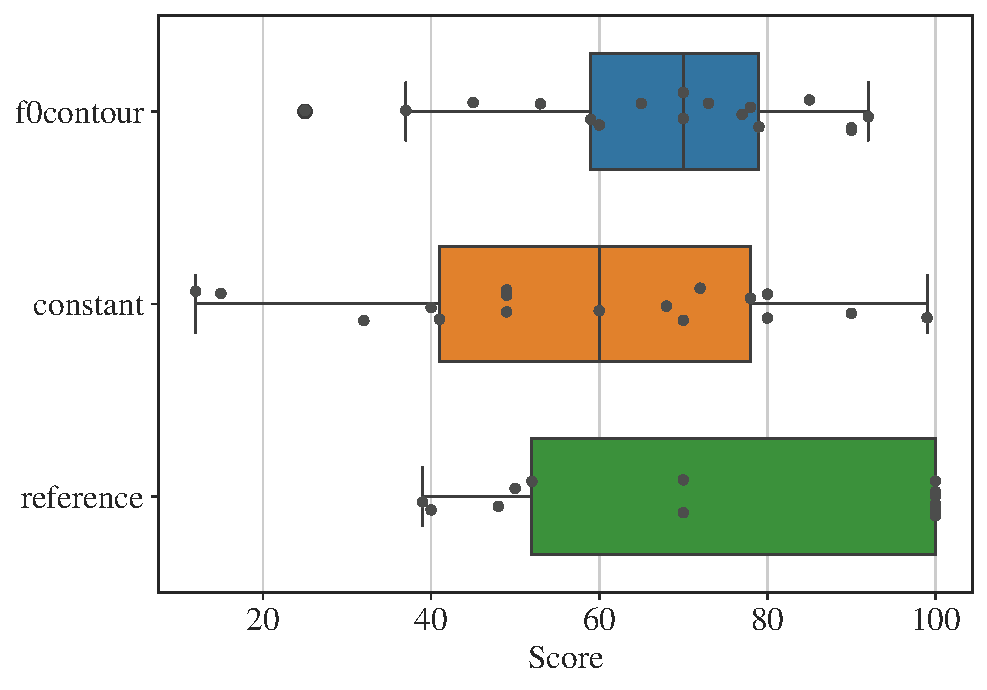
\includegraphics[width = 0.5\textwidth]{chapter7/vowels.pdf}
    \caption{Vowel synthesis results}
    \label{fig:vowels}
\end{figure}

\begin{table}[H]
    \centering
    \begin{tabular}{lccc}
        \hline
        & Reference & Constant $F_0$ & Contour $F_0$ \\
        \hline

        $\mu$ & 80.529 & 57.882 & 67.529 \\ %\cline{2-6}
        $\sigma^2$ & 25.229 & 25.017 & 19.174 \\
        $CI_{95\%}$ & $\pm$ 11.99 & $\pm$ 11.89 & $\pm$ 9.11 \\ \hline
    
    \end{tabular}
    \caption{Vowel synthesis results}
    \label{tab:vowelSynth}
\end{table}

From this, it is clear that the synthesized vowels generated with the $F_0$ contour generally performed with a higher mean score than the constant $F_0$ frequency, which is in line with the expectations. This is due to the fact that the $F_0$ contour being defined to simulate some sort of natural sounding prosody, which is able to generate a more natural sounding speech. From the pairwise t-test results shown in table \ref{tab:pairwiseVowel}, it is clear that the differences between the synthesized vowels are statistically significant, with p < 0.05. Despite this, all the stimuli have shown higher variance indicating that the quality of the synthesized vowels and the reference is not as consistent as the whispered-to-speech conversion tests.

\begin{table}[H]
    \centering
    \begin{tabular}{lcccc}
        \hline
        & Reference & Constant $F_0$ & Contour $F_0$ \\
        \hline
        Reference & - & 4.70e-02 & 4.95e-11 \\
        Constant $F_0$ & 4.70e-02 & - & 6.99e-11 \\
        Contour $F_0$ & 4.95e-11 & 6.99e-11 & - \\
        \hline
    \end{tabular}
    \caption{Pairwise P-Values for Vowel Synthesis}
    \label{tab:pairwiseVowel}
\end{table}


%\vspace*{12mm}
